\chapter{АРХИТЕКТУРА И ПРОЕКТИРОВАНИЕ}
\label{chap:arch_design}
\aftertitle

В данной главе рассматривается архитектура и проектирование системы анализа новостей. Проектирование системы основано на анализе рассмотренных решений и алгоритмов.

\section{Формулирование требований к системе анализа новостей}
В рамках данной работы разрабатывается сервис, позволяющий анализировать семантическое сходство пользовательских запросов и новостей за определенный промежуток времени с использованием нейронных сетей.

Были сформулированы следующие требования к системе:

\begin{enumerate}
    \item функциональные требования:
    \begin{enumerate}
        \item сервис должен предоставлять пользователю REST API для взаимодействия с сервисом;
        \item сервис должен предоставлять возможность семантического поиска новостей;
        \item сервис должен предоставлять возможность определять основные темы новостей за заданный промежуток времени;
        \item сервис должен предоставлять возможность расчёта корреляции количества новостей по заданным темам с предоставленными пользователем числовыми рядами;
    \end{enumerate}
    \item Требования к окружению:
    \begin{enumerate}
        \item Сервис должен работать на серверах под управлением ОС Linux;
        \item Сервис должен использовать GPU для ускорения работы нейронных сетей.
    \end{enumerate}
\end{enumerate}

\section{Пользовательские сценарии}
Основываясь на сформулированных функциональных требованиях к системе анализа новостей, были сформированы следующие пользовательские сценарии. Диаграмма прецедентов представлена на рисунке \ref{img:use-case-diagram}.

\begin{figure}[h]
    \centering
    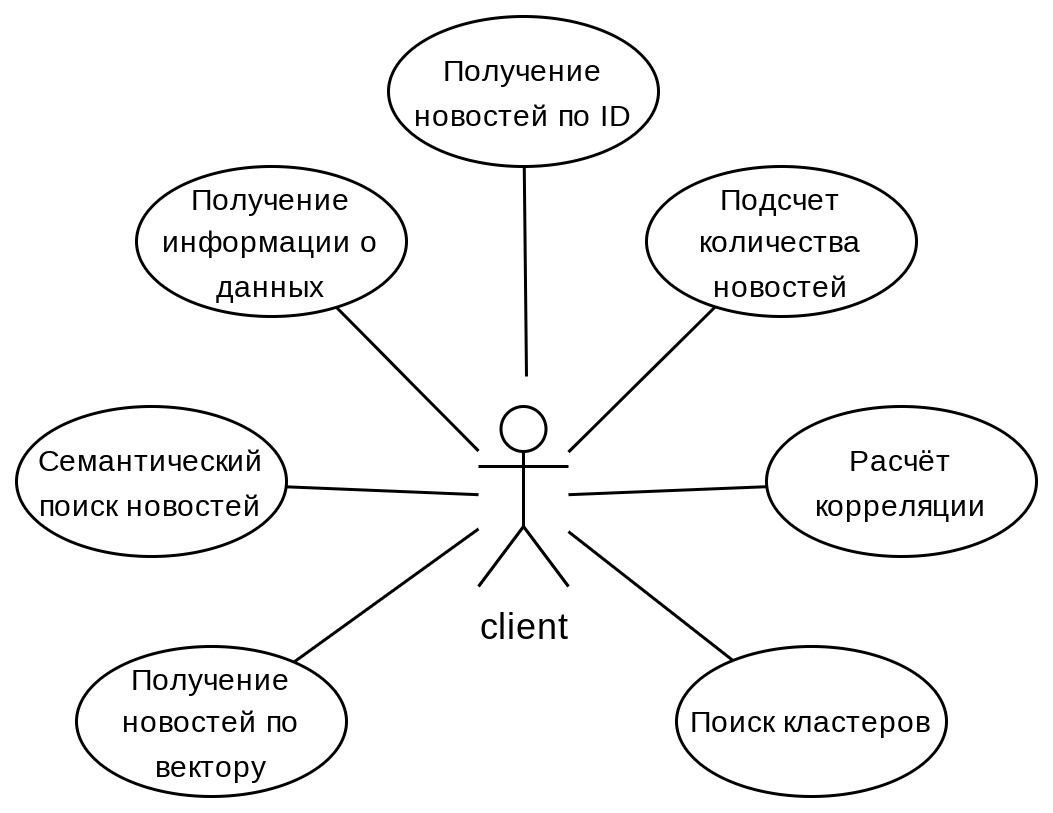
\includegraphics[width=\linewidth]{images/use-case-diagram.png}
    \caption{Диаграмма прецедентов системы}
    \label{img:use-case-diagram}
\end{figure}

Прецедент 1: Получение информации о данных.

Пользователь запрашивает информацию о датасете. В результате пользователь получает общую информацию о новостях: дату первой и последней новости в датасете, общее количество новостей.

Прецедент 2: подсчет количества новостей.

Пользователь запрашивает количество новостей. Для этого в запросе пользователь указывает обязательные параметры: границы временного интервала. Дополнительно пользователь может указать список интересующих тем новостей. В результате пользователь получает количество новостей за указанный временной интервал для каждой запрошенной темы (если они были представлены) и общее количество новостей за указанный временной интервал.

Прецедент 3: расчёт корреляции.

Пользователь запрашивает расчёт корреляции между количеством новостей и предоставленным пользователем временным рядом. Для этого пользователь указывает обязательные параметры: границы временного интервала, длительность окна, интересующую тему и список ~-- пользовательский временной ряд. В результате пользователь получает временной ряд ~-- корреляцию между количеством новостей и пользовательским временным рядом для каждого окна.

Прецедент 4: поиск кластеров.

Пользователь запрашивает кластеризацию новостей, т.е. определение основных тем новостей. Для этого пользователь указывает обязательные параметры: границы временного интервала. Дополнительно пользователь может указать параметры для алгоритма кластеризации. В результате пользователь получает список кластеров. Каждый кластер содержит список новостей, входящих в кластер.

Прецедент 5: Получение новостей по ID.

Пользователь запрашивает новость по ее ID. Для этого пользователь указывает обязательный параметр: ID новости. В результате пользователь получает данные о новости: ID, заголовок, дату и время публикации новости.

Прецедент 6: Получение новостей по вектору.

Пользователь запрашивает поиск ближайших новостей к заданному вектору. Пользователь указывает обязательные параметр: вектор и максимальное количество новостей, либо certainty для ограничения количества новостей. В результате пользователь получает список новостей, наиболее близких к указанному вектору. Каждая новость представлена следующими данными: ID, заголовком, датой и временем публикации новости.

Прецедент 7: Семантический поиск новостей.

Пользователь осуществляет семантический поиск новостей, т.е. получение новостей, наиболее близких к указанному текстовому запросу. Пользователь указывает обязательные параметр: текст запроса и максимальное количество новостей, либо certainty для ограничения количества новостей. В результате пользователь получает список новостей, наиболее близких к указанному запросу. Каждая новость представлена следующими данными: ID, заголовком, датой и временем публикации новости.

\section{Проектирование системы хранения данных}
Исходя из требований к сервису и пользовательских сценариев требуется определять извлекать из базы данных новости, относящиеся к определенным темам, задаваемым пользователем. Невозможно вручную разметить все новости, тем более, определить соответствие произвольным пользовательским запросам, поэтому необходимо применять методы машинного обучения для извлечения новостей, семантически близких к пользовательским запросам.

Для этого необходимо решить две задачи:
\begin{itemize}
    \item определение семантической близости новостей к запросу;
    \item извлечение некоторого количества самых семантически близких к запросу новостей.
\end{itemize}

Как было рассмотрено в главе \ref{chap:analysis}, для решения задачи определения семантической близости текстовой информации применяются различные эмбеддинги.

Имея векторное представление новостей и векторное представление пользовательского запроса, задача определения наиболее семантически близких новостей сводится к задаче поиска ближайшего соседа.

В случае, если количество элементов, среди которых осуществляется поиск ближайших соседей, невелико, то могут применяться такие хорошо известные алгоритмы, как KNN (метод k-ближайших соседей). В противном случае, если имеется очень большое количество элементов, требуется применение особых алгоритмов, которые позволяют решать эту задачу эффективно.

Это семейство алгоритмов называется ANN (approximate nearest neighbor), и существует ряд алгоритмов для решения этой задачи. В качестве примера можно привести библиотеку FAISS [\textbf{TODO:ссылка}], которая реализует несколько быстрых алгоритмов ANN.

Тем не менее, использование библиотеки FAISS не всегда удобно, потому что она является низкоуровневой библиотекой, предоставляющей базовую функциональность. При использовании хранилища данных к нему выдвигаются такие требования, как
\begin{itemize}
    \item поддержка CRUD (create, read, update, delete) операций ~-- хранилище данных должно эффективно реализовывать эти операции, потому что в случае с большим объемом данных перестройка всего индекса (как это было бы в случае с непосредственным применением FAISS) на каждую операцию модификации данных привела бы к крайней низкой производительности системы;
    \item поддержка горизонтальной масштабируемости ~-- хранилище должно обеспечивать возможность репликации на несколько узлов вычислительной системы для увеличения производительности, если производительности одного узла не хватает для обработки запросов с требуемой задержкой;
    \item поддержка классических операций поиска и фильтрации ~-- помимо операций поиска ближайших соседей в векторном пространстве, хранилище данных должно поддерживать выполнение типичных операций баз данных, таких как фильтрация, сортировка итп;
    \item служебные возможности, такие как авторизация и контроль доступа.
\end{itemize}

Для решения всех этих задач служит особый класс баз данных ~-- векторные базы данных также называемые векторными поисковыми движками. Эти системы представляют собой нереляционные базы данных, которые способны осуществлять операции поиска с учетом близости векторного представления хранимых данных.

Векторные базы данных применяются для решения таких задач, как
\begin{itemize}
    \item семантический поиск ~-- поиск документов (например, веб-страниц) не по совпадению ключевых слов, а по семантической близости; иными словами, с помощью векторных поисковых движков можно найти документ, релевантный запросу, даже если он не содержит слова, используемые в запросе;
    \item поиск похожих изображений, например, идентификация человека по лицу.
\end{itemize}

Таким образом, было решено использовать векторную базу данных в качестве основы для разрабатываемой в рамках данной работы системы, потому что использование текстовых эмбеддингов совместно с векторной базой данных позволяет извлекать из базы данных новости, относящиеся к определенным темам, задаваемым пользователем.

\subsection{Выбор векторной базы данных}

Существуют несколько реализаций векторных баз данных. Одними из наиболее популярных являются Milvus [\cite{milvus}], Pinecone [\cite{pinecone}] и Weaviate [\cite{weaviate}]. Было произведено сравнение популярных векторных баз данных, чтобы выбрать ту, которая подходит для реализации данного проекта. Сравнение основных характеристик рассматриваемых векторных баз данных приведено в таблице \ref{tab:vector-db-compare}.

\begin{table}[ht]
    \caption{Сравнение векторных баз данных}
    \label{tab:vector-db-compare}
    \begin{tabularx}{\textwidth}{|l|X|X|X|}
        \hline
        & Weaviate & Milvus & Pinecone \\
        \hline
        Open Source & Да & Да & Нет \\
        \hline
        Self-hosted & Да & Да & Нет, только в облаке \\
        \hline
        Гибридный поиск & Да & Да & Нет \\
        \hline
        Язык запросов & GraphQL & JSON &  ? \\
        \hline
        Ответы на вопросы и генеративный ИИ & Да & Нет & Да \\
        \hline
        Модули & Да & Да & Да \\
        \hline
        Встроенные векторизаторы & Да & Нет & Нет (?) \\
        \hline
    \end{tabularx}
\end{table}

Векторная база данных Milvus является популярным решением для эффективного хранения и поиска векторных данных. Она имеет следующие преимущества и недостатки. Преимущества:
\begin{enumerate}
    \item открытый исходный код: Milvus является проектом с открытым исходным кодом;
    \item self-hosted развертывание: Milvus предоставляет возможность быть развернутым на собственной инфраструктуре;
    \item эффективное хранение и поиск: Milvus предоставляет эффективные алгоритмы хранения и поиска векторных данных. Она специально разработана для обработки больших объемов данных и обеспечивает высокую скорость выполнения запросов;
    \item масштабируемость: Milvus предлагает горизонтальное масштабирование, позволяющее расширять систему с ростом объема данных;
    \item поддержка гибридного поиска: поиск может включать не только векторный поиск, но и классические операции фильтрации, сортировки и т.п.
\end{enumerate}

Недостатки векторной базы данных Milvus:
\begin{enumerate}
    \item необходимость реализации векторизации: Milvus не предоставляет встроенных модулей для векторизации текста или других типов данных, для использования Milvus для текстовых данных необходимо самостоятельно реализовывать модули векторизации и обеспечить взаимодействие с клиентами и Milvus;
    \item сложность настройки: Milvus может потребовать дополнительных усилий для настройки и оптимизации, особенно при работе с большими объемами данных; неоптимальная конфигурация может привести к снижению производительности или неправильным результатам поиска.
\end{enumerate}

Другой популярной векторной базой данных является Pinecone. Векторная база данных Pinecone является мощным инструментом для хранения, поиска и анализа векторных данных. Она имеет следующие преимуществ и некоторые недостатки. Преимущества:

\begin{enumerate}
    \item высокая производительность: Pinecone специально оптимизирована для обработки больших объемов векторных данных с высокой скоростью;
    \item масштабируемость: Pinecone предлагает горизонтальное масштабирование, что позволяет легко расширять систему с ростом объема данных;
    \item многофункциональность: Pinecone предлагает разнообразные функции для работы с векторными данными, включая поиск похожих векторов, ранжирование результатов, фильтрацию и трансформацию данных, также обладает гибкими возможностями для добавления пользовательских функций и алгоритмов.
\end{enumerate}

Недостатки:

\begin{enumerate}
    \item зависимость от облачной инфраструктуры: Pinecone предлагает только облачное решение, что означает, что для использования его необходимо полагаться на инфраструктуру облачных провайдеров;
    \item ограниченная гибкость настройки: Pinecone предлагает удобный интерфейс и простоту использования, но при этом может иметь ограниченные возможности настройки и оптимизации.
\end{enumerate}

Другой векторной базой данных является Weaviate. Weaviate - это open-source система поиска, основанная на семантике и искусственном интеллекте, которая действует как векторная и графовая база данных. Преимущества:
\begin{enumerate}
    \item открытый исходный код: Weaviate является проектом с открытым исходным кодом;
    \item self-hosted развертывание: Weaviate предоставляет возможность быть развернутым на собственной инфраструктуре;
    \item поддержка модулей векторизации: Weaviate поддерживает модули векторизации, что позволяет автоматически преобразовывать данные в векторы для дальнейшего анализа; weaviate предоставляет несколько готовых модулей, включая модуль векторизации текста, использующий нейронные сети на архитектуре "Трансформер".
    \item масштабируемость: Weaviate предлагает горизонтальное масштабирование, позволяющее расширять систему с ростом объема данных;
    \item поддержка графовых структур данных, что позволяет управлять сложными связями между объектами.
    \item поддержка гибридного поиска: поиск может включать не только векторный поиск, но и классические операции фильтрации, сортировки и т.п.
\end{enumerate}

Недостатки:
\begin{enumerate}
    \item могут возникнуть сложности при масштабировании для очень больших объемов данных;
    \item Weaviate менее популяерн, чем другие БД, такие как Milvus, могут возникнуть сложности в решении проблем.
\end{enumerate}

Исходя из рассмотренных преимуществ и недостатков, было решено выбрать векторную базу данных Weaviate для использования в разрабатываемой в рамках данной работы системы.

\section{Проектирование общей структуры системы}

Рассмотрим архитектуру системы анализа новостей и основные компоненты, из которых она состоит. Диаграмма архитектуры представлена на рисунке \ref{img:system-architecture}.

\begin{figure}[h]
    \centering
    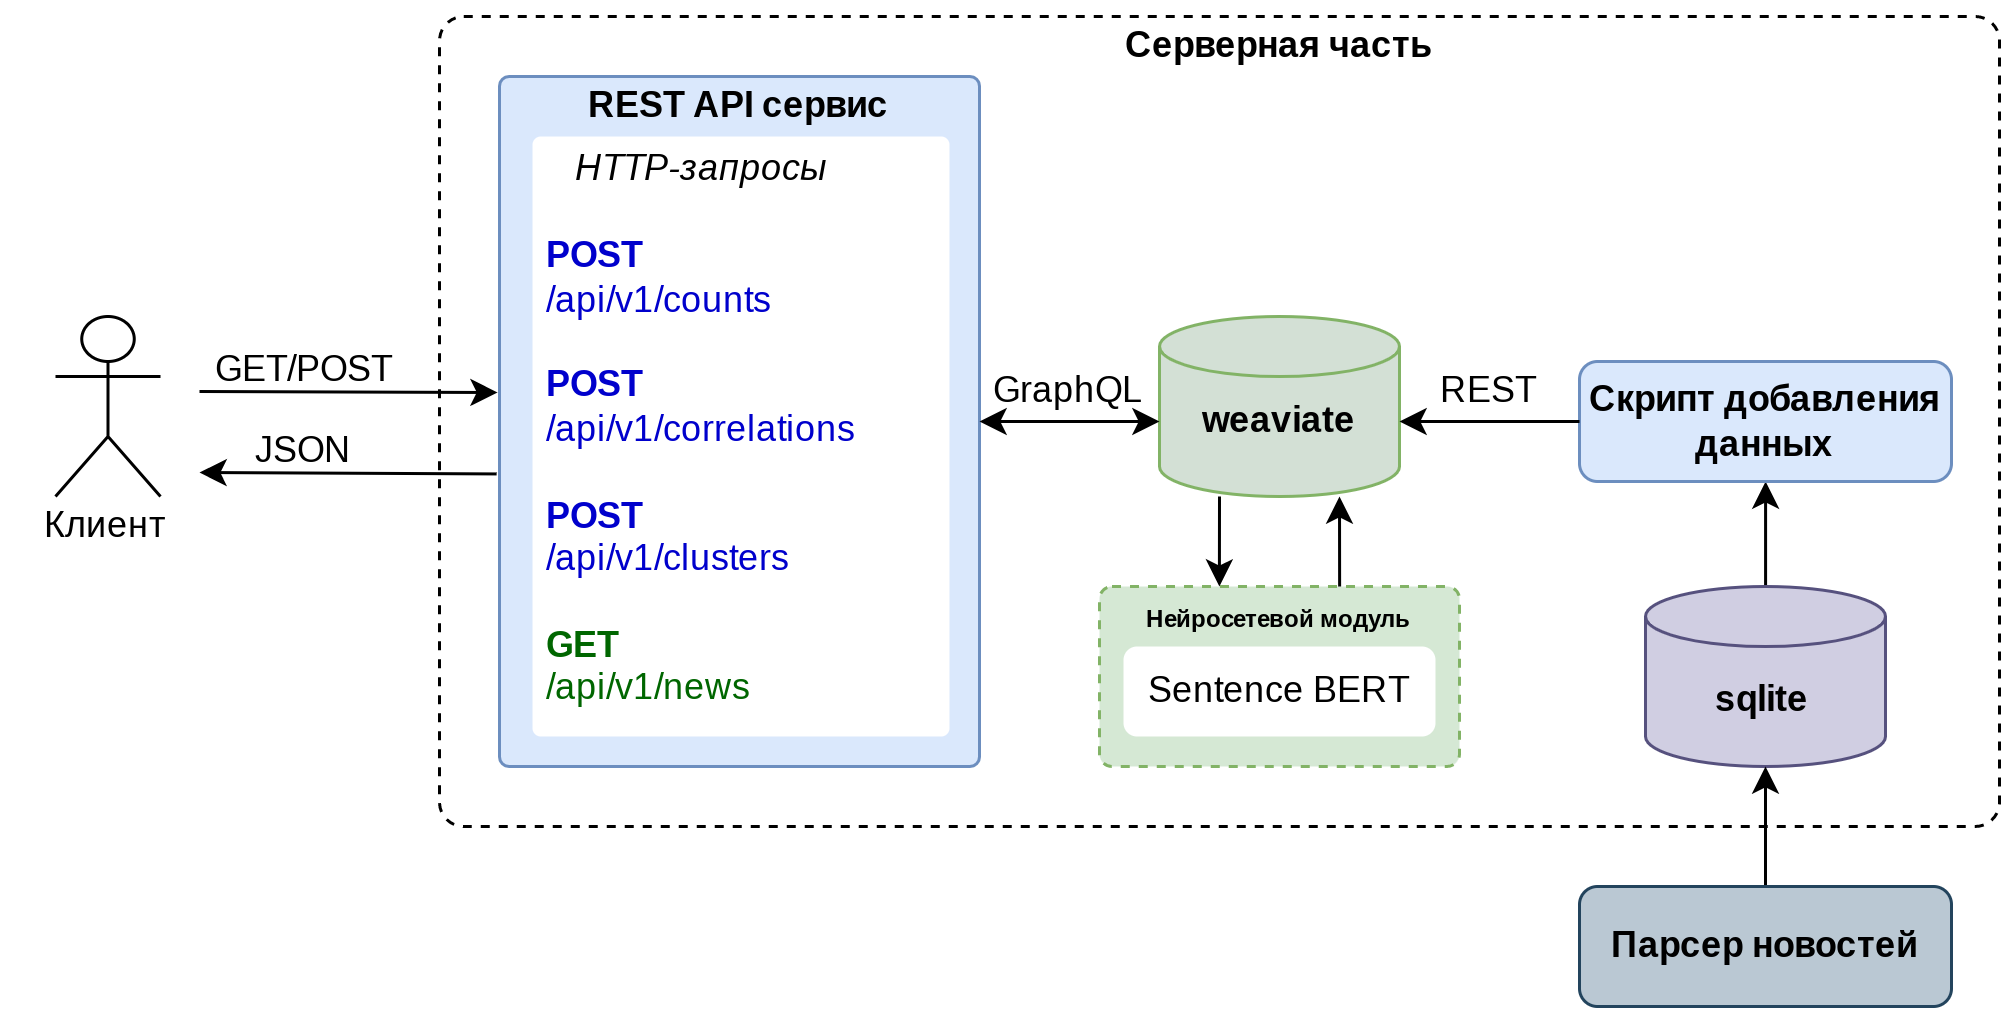
\includegraphics{images/system-architecture.png}
    \caption{Архитектура системы анализа новостей}
    \label{img:system-architecture}
\end{figure}

В основе системы, как было рассмотрено ранее, лежит векторная база данных Weaviate. weaviate выступает в качестве основного хранилища новостей и в качестве векторного поискового движка, который используется для извлечения новостей, относящиеся к определенным темам, задаваемым пользователем.

Для работы векторного семантического поиска, данные необходимо векторизовать. Для векторизации данных в Weaviate используются внешние модули. В данном случае, применяется стандартный модуль tex2vec-transformers, который осуществляет векторизацию текста с помощью нейронных сетей с архитектурой Трансформер.

Система представляет собой RESTful сервис, таким образом, необходим модуль, осуществляющий взаимодействие с клиентами с помощью REST. Этот модуль предоставляет внешнее REST-API сервиса и реализует основную логику сервиса, выполняя такие задачи как поиск новостей, расчет кросс-корреляции, кластеризацию новостей и другие. Для получения данных сервис обращается к базе данных Weaviate, используя язык запросов к данным GraphQL.

Для упрощения развертывания сервиса на узлах вычислительного кластера, применяются Docker контейнеры. Основные компоненты системы: Weaviate, модуль векторизации Weaviate и сервис развернуты в отдельных Docker-контейнерах.

В дополнении к рассмотренным компонентам системы, которые используются для функционирования сервиса, имеется подсистема получения новостей. Подсистема получения новостей используется для парсинга, обработки и сохранения новостей с целью дальнейшего использования сервисом. Подсистема получения новостей состоит из следующих компонентов:
\begin{itemize}
    \item парсер новостей ~-- скрипт, который непрерывно читает и сохраняет новости в sqlite базу данных;
    \item sqlite база данных ~--- промежуточное хранилище считанных новостей;
    \item скрипт для добавления данных переносит новости из промежуточного хранилища в sqlite в Weaviate; в процессе добавления новостей в БД Weaviate, происходит их векторизация.
\end{itemize}
